\documentclass[12pt,a4paper]{article}

\usepackage[onehalfspacing]{setspace}
\usepackage{natbib}
 
\usepackage{float}
%f�r feststellen der figures und tables [H] dranschreiben
\usepackage{siunitx}
%\SI{value}{unit commands} \SI{value}[pre-unit]{unit commands}
%\usepackage{units}
%wird so benutzt: 
%\unit[value/Zahl]{dimension/Einheit} oder 
%\unitfrac[value/Zahl]{dimension/Einheit num/Z�hler}{dimension/Einheit denum/Nenner} oder
%\nicefrac[fontcommand/Schriftart]{dimension/Einheit num/Z�hler}{dimension/Einheit denum/Nenner}
\usepackage{amssymb}
\usepackage{caption}
\usepackage{subcaption}

\usepackage{hyperref}

\usepackage[left=2cm,right=2cm,top=2cm,bottom=2cm]{geometry}
\usepackage[latin9]{inputenc}
\usepackage[ngerman]{babel}
\usepackage[T1]{fontenc}
\usepackage{lmodern}
\usepackage{amsmath}
\usepackage{graphicx}
\usepackage{textcomp}




\begin{document}

%deckblatt erstellen.

\begin{titlepage}

\begin{center}
% Oberer Teil der Titelseite:

\includegraphics[width=0.75\textwidth]{logo.png}\\[1cm]    	%Logo 

\textsc{\LARGE Bergische Universit\"at Wuppertal}\\[1.5cm]	%Institution

\textsc{\Large Fortgeschrittenen Praktikum}\\[0.5cm]				%Projekt


\newcommand{\HRule}{\rule{\linewidth}{0.5mm}}
\HRule \\[0.4cm]
{ \huge \bfseries Rutherford\\ Streuung von $\alpha$-Teilchen}\\[0.4cm]				%Titel

\HRule \\[1.5cm]

% Author und Tutor
\begin{minipage}{0.4\textwidth}
\begin{flushleft} \large
\emph{Verfasser:}\\
Henrik \textsc{J�rgens} \\
Frederik \textsc{Strothmann} \\
\end{flushleft}
\end{minipage}
\hfill
\begin{minipage}{0.4\textwidth}
\begin{flushright} \large
\emph{Tutoren:} \\
Max \textsc{Mustermann} \\
Max \textsc{Mustermann} \\
\end{flushright}
\end{minipage}

\vspace{1cm}

\begin{table}[H]
\centering
\begin{tabular}{|l|}
\hline \textbf{Abstract: } \\
Ziel des Versuches ist es, die Wechselwirkung von $\alpha$-Teilchen mit Materie zu untersuchen.\\
Die Aspekte Streuwinkel, Reichweite, Kernladung und Absorbtionsverhalten werden thematisiert.\\
\hline 
\end{tabular}
\end{table} 

\vspace{1cm}

\begin{table}[H]
\centering
\begin{tabular}{|c|c|c|}
\hline Dies & ist & ein \\ 
\hline Platz- & halter & f�r \\ 
\hline die & bewertungs & Tabelle \\ 
\hline 
\end{tabular} 
\end{table}

\vfill

% Unterer Teil der Seite/Datum
{\large \today}

\end{center}

\end{titlepage}

\newpage
\tableofcontents
\newpage

\bibliographystyle{plain}


\section{Einleitung}
%einleitung zu dem experiment.
%auf die einstellungen, die vor dem versuch gemacht werden, eingehen, oder auf eine anleitung dazu verweisen.
%---------------------------------------------------------------------------------------------
%hinter der einleitung kann der allgemeine theoretische hintergrund in einer zus�tzlichen section erkl�rt werden
In diesem Versuch werden Oberfl�chen verschiedener Proben mittels Rasttunnelmikroskopie auf deren Gitterstruktur und morphologische Eigenschaften untersucht. Elektronendichte, Oberfl�chenrauheit und die atomare Gitterstruktur k�nnen mit dem Rastertunnelmikroskop (RTM) analysiert werden. Der quantenmechanische Tunneleffekt wird genutzt, um leitende Materialien zu untersuchen. Indem zwischen einer einatomigen Platin-Iridum-Elektrode und der zu untersuchenden Probe eine Potentialdifferenz angelegt wird, kommt es abh�ngig von der Entfernung der Pt-Ir-Elektrode zur Probe und dessen Elektronendichte zu einem Tunnelstrom, welcher R�ckschl�sse auf die Struktur der Probe erlaubt. Die Elektronendichte der Oberfl�che kann durch systematisches Abrastern der Probe erfasst werden, sodass mithilfe verschiedener Modi (CC und CH: Constant Current und Constant Height) ein Bild der Materialoberfl�che entsteht.
\section{Theorie}
% Es sollen die wichtigsten theoretischen Formeln und Zusammenh�nge einmal ausf�hrlich erkl�rt werden
Es werden die theoretischen Grundlagen zur Bestimmung der Lebensdauer von Myonen besprochen.

\subsection{Standardmodell}
Das Standartmodell der Teilchenphysik drei der vier Grundlegenden Wechselwirkungen (WW), die schwache WW, die elektromagnetische WW und die Starke WW.
Die Kr�fte wechselwirken �ber Vektorbosonen, welche eine ganzzahligen Spin haben.
In Tabelle \ref{tab:ww} ist eine �bersicht der drei Kr�fte zu sehen.

\begin{table}[H]
\caption{In der Tabelle sind die Grundlegenden WW (au�er der Gravitation) und ihre Eigenschaften aufgetragen (entnommen \cite{povh} Seite 274)}
\label{tab:ww}
\centering
\begin{tabular}{|c|c|c|c|c|}
\hline Wechselwirkung & koppelt an & Austauschteilchen & $\frac{m_0}{GeV}$ & J$^P$ \\ 
\hline stark & Farbe & 8 Gluonen (g) & 0 & 1$^-$ \\ 
\hline elektromagnetisch & elektrische Ladung & Photon ($\gamma$) & 0 & 1$^-$ \\ 
\hline schwach & schwache Ladung & W$^\pm$, Z$^0$ & $\approx 10^2$ & 1 \\ 
\hline 
\end{tabular} 
\end{table}
Neben den Bosonen gibt es noch zwei weitere Fundamentale Teilchenarten die Quark und die Leptonen welche die Grundbausteine der Materie darstellen.
Beide geh�ren zu den Fermionen, haben also einen halbzahligen Spin. Leptonen und Quarks werden mit aufsteigender Masse in drei Generationen aufgeteilt.
In Tabelle \ref{tab:fermi} sind Quarks und Leptonen mit ihren Eigenschaften dargestellt.

\begin{table}[H]
\caption{�bersicht der Grundlegenden Eigenschaften von Quarks und Leptonen}
\label{tab:fermi}
\centering
\begin{tabular}{|p{2cm}|p{2cm}|p{2cm}|p{1cm}|p{3.5cm}|p{1cm}|}
	\hline
	Fermionen & \hspace{0.25cm} Familie \newline 1 \hspace{0.3cm} 2 \hspace{0.3cm} 3                                               & elektrische Ladung    & Farbe  & schwacher Isospin \newline rechtsh. \hspace{0.5cm} linksh. & Spin \\ \hline
	Leptonen  & $\nu_e$ \hspace{0.17cm} $\nu_\mu$ \hspace{0.17cm} $\nu_\tau$ \newline e \hspace{0.3cm} $\mu$ \hspace{0.3cm} $\tau$ & \hspace{0.6cm} 0 \newline  \hspace*{0.6cm} -1      & ------ & 1/2 \hspace{1.5cm} --- \newline \hspace*{2.4cm} 0          & 1/2  \\ \hline
	Quarks    & u \hspace{0.3cm} c \hspace{0.3cm} t \newline d \hspace{0.3cm} s \hspace{0.3cm} b                                   & \hspace*{0.2cm} +2/3 \newline \hspace*{0.3cm} -1/3 & r,g,b  & 1/2 \hspace{1.64cm} 0 \newline \hspace*{2.4cm} 0           & 1/2  \\ \hline
\end{tabular} 
\end{table}


\section{Versuchsaufbau}
%skizze zum versuchsaufbau (oder foto) einf�gen,   es muss erkl�rt werden wie das ganze funktioniert und welche speziellen einstellungen verwendet wurden (z.b. welche kn�pfe an den ger�ten f�r die messung verdreht wurden)
F�r den Versuch werden zwei verscheiden Vakuumkammern verwendet. Die erste Kammer  ist eine Rutherford-Streukammer, eine schematische Skizze ist in Abb. \ref{fig:kammer} zu sehen. Die Streukammer besteht aus einer Vakuumkammer, mit durchsichtigem Deckel. Ein Barometer, ein Bel�ftungsventil und ein Ventil mit Anschluss an die Vakuumpumpe sind an den Absperrhahn (3) angeschlossen. Der Halbleiterdetektor mit Kollimator (12,12.1) ist von innen an einer BNC-Buchse (2.1) montiert. Von au�en ist ein Vorverst�rker angeschlossen, die Daten werden von einem Digitalz�hler, der an einen Computer angeschlossen ist ausgelesen (siehe Abb. \ref{fig:aufbau}). Der Deckel der Streukammer hat einen Schwenkarm (7), an dem das $^{241}$Am-Pr�parat (7.1) , verschiedene Rahmen mit SpaltkKollimatoren (9) und Metallfolien (10) angebracht werden k�nnen. �ber einen Knopf (4) ist der Schwenkarm drehbar, der Winkel ist dabei �ber eine Skala (8) ablesbar. Zur Verf�gung stehen Spalte mit 1m und 5mm Breite sowie eine Goldfolie mit 2$\mu$m und eine Aluiminiumfolie mit 7$\mu$m Dicke.

\begin{figure}[H]
	\centering
  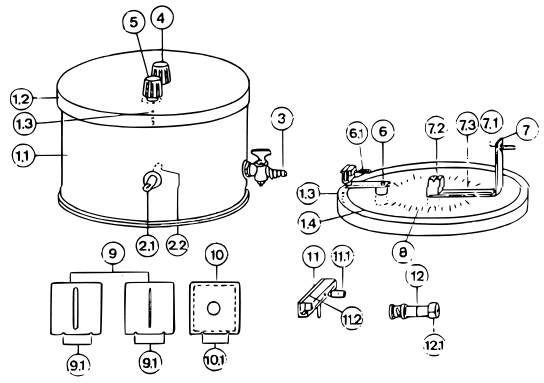
\includegraphics[scale=0.4]{streukammer.png}
	\caption{Schematischer Aufbau des Streukammer}
	\label{fig:kammer}
\end{figure}


\begin{figure}[H]
	\centering
  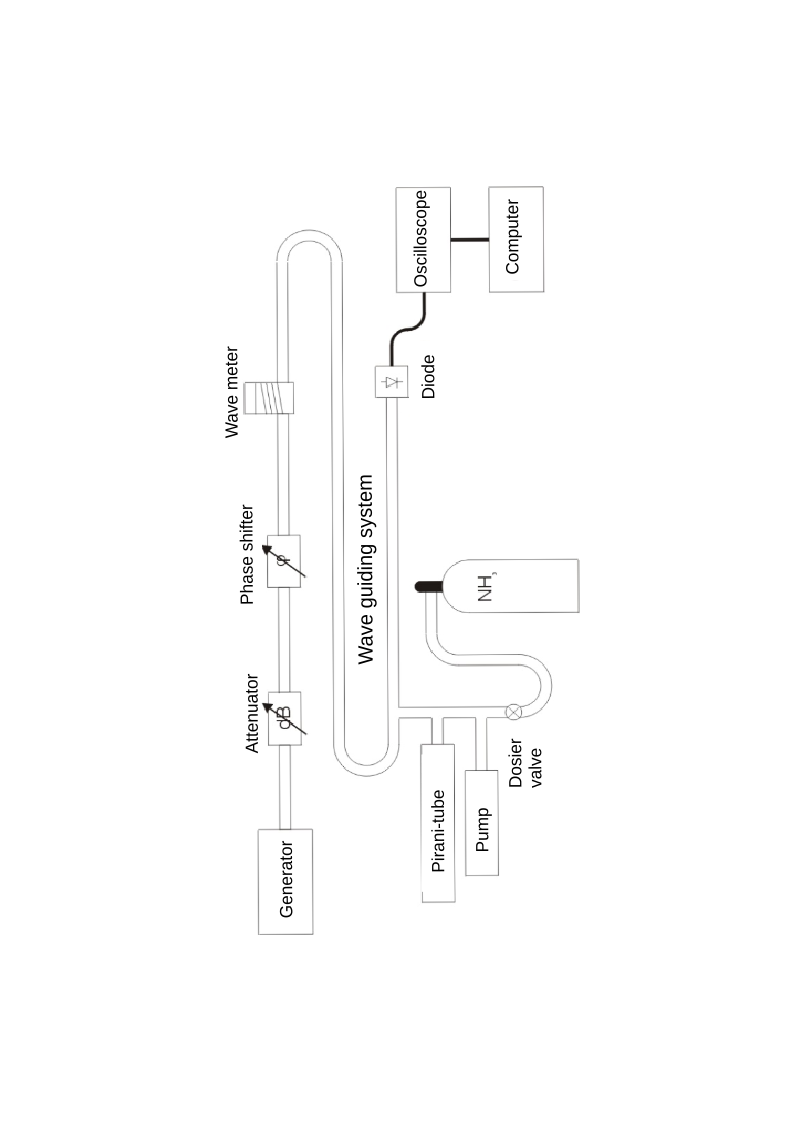
\includegraphics[scale=0.4]{aufbau.png}
	\caption{Schematischer Aufbau des Versuchsaufbaus}
	\label{fig:aufbau}
\end{figure}

Die zweite Kammer ist eine Vakuumkammer, mit einer optischen Bank, zu befestigen der radioaktiven Quelle. Sie wird f�r die Bestimmung der Reichweite von $\alpha$-Strahlung und die Untersuchung von Absorbtion durch verschiedenen Medien verwendet. Der Detektor ist an einen PC angeschlossen mit dem die Messdaten aufgenommen werden.
\section{Versuchsdurchf�hrung und Auswertung}
%die messwerte in !�bersichtlichen! tabellen angegeben
%zu viele kleine tabellen in gro�e tabellen �berf�hren!
%zu gro�e tabellen mit dem [scale]-befehl scalieren oder (falls zu lang) in zwei kleinere tabellen aufteilen
%(wichtig) vor !jeder! tabeelle sagen, was gemessen wurde und wie die fehler gew�hlt wurden und ausreichend !erkl�ren!, !warum! wir unsere fehler grade so gew�hlt haben

%zuerst !alle! errechneten werte entweder in ganzen s�tzen aufz�hlen, oder in tabellen (�bersichtlicher) dargestellen, sowie auf die verwendeten formeln verweisen (die referenzierung der formel kann in der �berschrift stehen)
%kurz erw�hnen (vor der tabelle), warum wir das ganze ausrechnen bzw. was wir dort ausrechnen
%danach histogramme und plots erstellen, wobei wenn m�glich funktionen durch die plots gelegt werden (zur not k�nnen auch splines benutzt werden, was aber angegeben werden muss)
%bei fits immer die funktion und das reduzierte chiquadrat mit angegeben, wobei auf verst�ndlichkeit beim entziffern der zehnerpotenzen geachtet werden muss z.b. f(x)=(wert+-fehler)\cdot10^{irgendeine zahl}\cdot x + (wert+-fehler)\cdot10^{irgendeine zahl}
%bei jedem fit erkl�ren, nach welchem zusammenhang gefittet wurde und warum!
%bei plots darauf achten, dass die achsenbeschriftung (auch die tics) die richtige gr��e haben und die legende im plot nicht die messwerte verdeckt
%kurz die aufgabenstellung abgehandeln

Der Versuch besteht aus f�nf Teile, welche im folgendem beschrieben und ausgewertet werden.

\subsection{Inbetriebnahme}
Vor dem einstellen des SQUID muss das Dewar-Gef�� in ein Bad von fl�ssigem Stickstoff getaucht werden, damit der Sensor nicht durch Feuchtigkeit zerst�rt wird und die Supraleitung nicht unterbrochen wird. Das Bad von fl�ssigem Stickstoff muss eventuell w�hrend dem Versuch nachgef�llt werden. Der Abk�hlprozess dauert ca. 20 min, danach k�nnen Messungen gestartet werden. Zu erst soll die Amplitude I$_{rf}$ (VCA, voltage controlled atteuator) und die Auslesefrequenz (VCO voltage controlled oscillator) des rf-Signals so ein maximales Signal-zu-Rausch-Verh�ltnis von U($\Phi$) erreicht wird. F�r die Einstellungen wird der Testmodus, mit eingeschaltetem Generator verwendet. Zu erst wird f�r VCA ein Werte von 900 eingestellt.
% Kapazit�ts- und Widerstandsangaben hinzuf�gen
Dann wird der VCO Wert zwischen 0 und 4095 so variiert, das m�glichst deutlich ein Dreiecksignal zu sehen ist. Der VCA Wert wird nun nochmal variiert um das Signal weiter zu optimieren.

%  Bild und die Werte einf�gen

F�r die Einstellung des Arbeitspunkts wird das Offsets kalibriert. Das SQUID wird im Messmodus betrieben um die zeitliche Magnetfeld�nderung auf dem Oszilloskop zu beobachten. Es wird ein Kompensations-Widerstand von 20k$\Omega$ gew�hlt. Falls das Offset richtig eingestellt ist sollten keine Peaks auf dem Oszilloskop zu sehen sein. Falls Peaks nach oben zu sehen sind, ist das Offset zu hoch eingestellt. Bei Peaks, die nach unten zeige, ist das Offset zu niedrig eingestellt.

% Auswertung + Bilder + weiterf�hrende Analysen(50Hz Rauschen)

\subsection{Empfindlichkeit des SQUID}
Zur Untersuchung der Empfindlichkeit wird das SQUID im Messmodus betrieben. Um einen ersten Eindruck der Empfindlichkeit zu bekommen wurde .......................................

% kurze beschreibund der beobachungen + Bilder

F�r eine quantitative Bestimmung der Empfindlichkeit des SQUIDs wurde mit einer Spule Magnetfelder bekannter st�rke erzeugt. Um bei der Messung eine m�glichst hohe Empfindlichkeit zu haben wird ein Widerstand von 20k$\Omega$ verwendet. 

% messergebnisse und auswertung

\subsection{Kalibrierung}
F�r die weiteren Messungen muss der Sensor zuerst kalibriert werden, um as dem Signal die st�rke des Magnetfeldes bestimmen zu k�nnen. Es soll auch die Empfindlichkeit des SQUID in Abh�ngigkeit des R�ckkopplungswiderstandes gemessen werden. Zuerst wird f�r einen festen Widerstand das Magnetfeld in Abh�ngigkeit der Str�me in der Leiterschleife untersucht. Es werden Str�me zwischen \SI{0}{mA} und \SI{90}{mA} verwendet. 

% messdaten und widerstand angeben

Aus den H�hen der Plateaus und den jeweiligen Str�men kann eine lineare Regerssion durchgef�hrt werden, um den Zusammenhang zwischen dem Strom in der Leiterschleife und der Spannung her zu stellen.

%messdaten + bilder

Die Messung wird f�r die anderen Widerst�nde wiederholt (siehe Abb. ??)

\subsection{Aufzug}
In diesem Versuchsteil soll das Magnetfeld der Aufz�ge untersucht werden. Dabei wird der Aufzug als Dipol angenommen, da das Gegengewicht eine nat�rliche Magnetisierung besitzt. Durch die Messung soll die z-Komponente des Dipols bestimmt werden.

\subsection{Magnetisierungskurve von Gadolinium und Curie-Temperatur}
In diesem Versuchsteil soll aus der Magnetisierungskurve von Gadolinium die Curie-Temperatur abgelesen werden. Zuerst wird das Gadolinium unter T$_c$ gek�hlt und magnetisiert. Die Temperatur wird dabei mit einem PT1000 Element gemessen.
\subsection{Diskussion}
%(immer) die gemessenen werte und die bestimmten werte �ber die messfehler mit literaturwerten oder untereinander vergleichen
%in welchem fehlerintervall des messwertes liegt der literaturwert oder der vergleichswert?
%wie ist der relative anteil des fehlers am messwert und damit die qualit�t unserer messung?
%in einem satz erkl�ren, wie gut unser fehler und damit unsere messung ist
%kurz erl�utern, wie systematische fehler unsere messung beeinflusst haben k�nnten
%(wichtig) zum schluss ansprechen, in wie weit die ergebnisse mit der theoretischen vorhersage �bereinstimmen
%--------------------------------------------------------------------------------------------
%falls tabellen mit den messwerten zu lang werden, kann die section mit den messwerten auch hinter der diskussion angef�gt bzw. eine section mit dem anhang eingef�gt werden.

Um die Diskussion konsistent zu halten, werden nur die Messdaten unserer Kommilitonen Diskutiert. 

Beim Sputtern wurden Prismen mit 5 verschiedenen Dicken Goldschichten erstellt 18nm, 27nm, 36nm, 45nm und 63nm. Bevor die Messung begonnen werde konnten, musste die Messapparatur justiert werden. Zuerst wurde die Position des Detektors justiert, dabei wurde eine Offset von 1,9(2) $^\circ$ bestimmt. Damit ergibt sich die Nulllage bei 181,9 $^\circ$. Bei der Bestimmung des Winkels, bei dem parallel bzw. senkrecht Polarisiertes Licht erzeugt wird, ergab sich ein Winkel von 89$^\circ$. Entsprechend ist der Winkel f�r senkrecht polarisiertes Licht -1$^\circ$. Der Brechungsindex des Prismas wurde �ber den Brewsterwinkel bestimmt, dabei ergab sich ein Wert von n$_{prisma}$=1.51. Nach der Justierung konnte die R$_p$/R$_s$-Kurve aufgenommen werden. Bei den allen Schichtdicken au�er der 63nm Schicht ist die Plasmonenresonanzkurve deutlich zu sehen. �ber eine Fit konnte der Resonanzwinkel bestimmt werden, aus welchem die Wellenzahl der Oberfl�chenplasmonen bestimmt werden konnte. Es ergab sich eine maximale Wellenzahl von 9,96(11) $\cdot$ 10$^6$ m$^{-1}$.


\section{Conclusion}
%im fazit nochmal alles zusammenfassen und den verlauf der messung absch�tzen
%gravierende sytematische probleme bei den messungen nochmal betonen und die wertigkeit unserer ergebnisse einordnen

In the first part of the experiment the 39 peaks of the nH$_3$ spectrum where measured and there relative absorption coefficients where calculated. In the second part the quadrupole moment where determined with a value of 5.02(9), with a deviation of 17.53\%. In the last part the broadening of the peaks according to the pressure was determined with 28 witch is a good measurement. 



\bibliography{ref}

\end{document}